\documentclass[nohyper,justified]{tufte-handout}\usepackage[]{graphicx}\usepackage[]{color}
%% maxwidth is the original width if it is less than linewidth
%% otherwise use linewidth (to make sure the graphics do not exceed the margin)
\makeatletter
\def\maxwidth{ %
  \ifdim\Gin@nat@width>\linewidth
    \linewidth
  \else
    \Gin@nat@width
  \fi
}
\makeatother

\definecolor{fgcolor}{rgb}{0.345, 0.345, 0.345}
\newcommand{\hlnum}[1]{\textcolor[rgb]{0.686,0.059,0.569}{#1}}%
\newcommand{\hlstr}[1]{\textcolor[rgb]{0.192,0.494,0.8}{#1}}%
\newcommand{\hlcom}[1]{\textcolor[rgb]{0.678,0.584,0.686}{\textit{#1}}}%
\newcommand{\hlopt}[1]{\textcolor[rgb]{0,0,0}{#1}}%
\newcommand{\hlstd}[1]{\textcolor[rgb]{0.345,0.345,0.345}{#1}}%
\newcommand{\hlkwa}[1]{\textcolor[rgb]{0.161,0.373,0.58}{\textbf{#1}}}%
\newcommand{\hlkwb}[1]{\textcolor[rgb]{0.69,0.353,0.396}{#1}}%
\newcommand{\hlkwc}[1]{\textcolor[rgb]{0.333,0.667,0.333}{#1}}%
\newcommand{\hlkwd}[1]{\textcolor[rgb]{0.737,0.353,0.396}{\textbf{#1}}}%

\usepackage{framed}
\makeatletter
\newenvironment{kframe}{%
 \def\at@end@of@kframe{}%
 \ifinner\ifhmode%
  \def\at@end@of@kframe{\end{minipage}}%
  \begin{minipage}{\columnwidth}%
 \fi\fi%
 \def\FrameCommand##1{\hskip\@totalleftmargin \hskip-\fboxsep
 \colorbox{shadecolor}{##1}\hskip-\fboxsep
     % There is no \\@totalrightmargin, so:
     \hskip-\linewidth \hskip-\@totalleftmargin \hskip\columnwidth}%
 \MakeFramed {\advance\hsize-\width
   \@totalleftmargin\z@ \linewidth\hsize
   \@setminipage}}%
 {\par\unskip\endMakeFramed%
 \at@end@of@kframe}
\makeatother

\definecolor{shadecolor}{rgb}{.97, .97, .97}
\definecolor{messagecolor}{rgb}{0, 0, 0}
\definecolor{warningcolor}{rgb}{1, 0, 1}
\definecolor{errorcolor}{rgb}{1, 0, 0}
\newenvironment{knitrout}{}{} % an empty environment to be redefined in TeX

\usepackage{alltt}
\usepackage{mathtools}
%%\usepackage{marginnote}
%%\usepackage[top=1in, bottom=1in, outer=5.5in, inner=1in, heightrounded, marginparwidth=1in, marginparsep=1in]{geometry}
\usepackage{enumerate}
%% mess with the fonts
%%\usepackage{fontspec}
%%\defaultfontfeatures{Ligatures=TeX} % To support LaTeX quoting style
\usepackage[T1]{fontenc}
\usepackage[utf8]{inputenc}
% For package xtable
\usepackage{booktabs}  % Nice toprules and bottomrules
\heavyrulewidth=1.5pt  % Change the default to heavier lines
\usepackage{longtable} 
%%\usepackage{tabularx}  % To control the width of the table

% this should make caption font bold.
%%\usepackage{xstring}
%%\usepackage{etoolbox}

%%\usepackage{url}

%% xetex only \usepackage{breakurl}
\usepackage{float} % for fig.pos='H'
%%\usepackage{wrapfig}
%%\usepackage{tikz}


\usepackage{colortbl,xcolor}
\makeatletter
% Paragraph indentation and separation for normal text
\renewcommand{\@tufte@reset@par}{%
  \setlength{\RaggedRightParindent}{0pc}%
  \setlength{\JustifyingParindent}{0pc}%
  \setlength{\parindent}{0pc}%
  \setlength{\parskip}{3pt}%
}
\@tufte@reset@par

% Paragraph indentation and separation for marginal text
\renewcommand{\@tufte@margin@par}{%
  \setlength{\RaggedRightParindent}{0pc}%
  \setlength{\JustifyingParindent}{0pc}%
  \setlength{\parindent}{0pc}%
  \setlength{\parskip}{2pt}%
}
\makeatother
\makeatletter
\title{Descriptive Statistics -- Associations}
\author{Kate Davis}
\makeatother

\newcommand{\dev}[1] {Dev_{\bar{#1}}}
\IfFileExists{upquote.sty}{\usepackage{upquote}}{}
\begin{document}
\widowpenalty=10000 
\clubpenalty=10000



\section{Association of Hours Studied to Exam Grade}
Six students enrolled in a reading section of organic chemistry are preparing for their first exam. How are the hours each student studied and their exam grade associated?

\section{Scatterplot}
A \textbf{Scatterplot} of exam grade by hours studied variables shows the relationship on the same observation, in this case, student. 
\begin{knitrout}
\definecolor{shadecolor}{rgb}{0.969, 0.969, 0.969}\color{fgcolor}\begin{figure}

{\centering 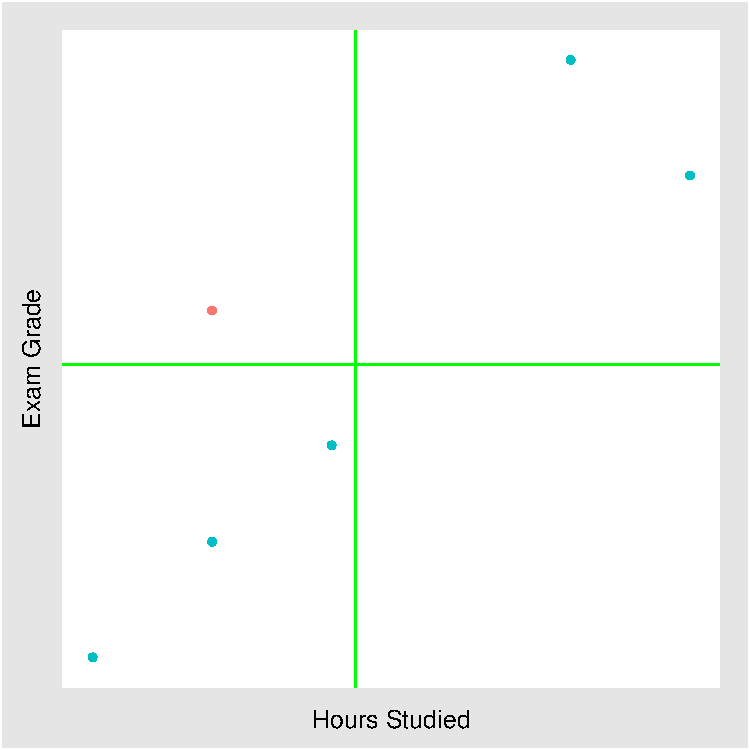
\includegraphics[width=\maxwidth]{figure/graphics-scatterplotsxy-1} 

}

\caption[A scatterplot of Hours Studied v Exam Grade shows a possible linear relationship]{A scatterplot of Hours Studied v Exam Grade shows a possible linear relationship}\label{fig:scatterplotsxy}
\end{figure}


\end{knitrout}



% latex table generated in R 3.1.2 by xtable 1.7-4 package
% Thu Feb 26 11:17:42 2015
\begin{table}[ht]
\centering
\begin{tabular}{rrr}
  \hline
 & examgrade & studyhours \\ 
  \hline
Min. & 57.0 & 1.0 \\ 
  1st Qu. & 64.2 & 2.0 \\ 
  Median & 71.5 & 2.5 \\ 
  Mean & 72.2 & 3.2 \\ 
  3rd Qu. & 80.2 & 4.5 \\ 
  Max. & 88.0 & 6.0 \\ 
  Sum Sq Deviation & 686.6 & 18.6 \\ 
  Variance & 114.4 & 3.1 \\ 
  Standard Deviation & 10.7 & 1.8 \\ 
   \hline
\end{tabular}
\caption{Summary Statistics Hours Studied and Grades} 
\end{table}


% latex table generated in R 3.1.2 by xtable 1.7-4 package
% Thu Feb 26 11:17:42 2015
\begin{table}[ht]
\centering
\begin{tabular}{rp{1.5cm}p{1.5cm}p{1.5cm}p{1.5cm}}
  \toprule
 & Exam Grade & Hours Studied & $\dev{x} hours$ & $\dev{y} grade$ \\ 
  \midrule
A & 82 & 6 & 9.8 & 2.8 \\ 
   \rowcolor[gray]{0.95}B & 63 & 2 & -9.2 & -1.2 \\ 
  C & 57 & 1 & -15.2 & -2.2 \\ 
   \rowcolor[gray]{0.95}D & 88 & 5 & 15.8 & 1.8 \\ 
  E & 68 & 3 & -4.2 & -0.2 \\ 
   \rowcolor[gray]{0.95}F & 75 & 2 & 2.8 & -1.2 \\ 
   \bottomrule
Total & 433.0& 19.0&  0.0&  0.0  \\ 
\rowcolor[gray]{0.95}Total/N &  $\bar{x}=10.7$ & $\bar{y}= 1.8$ & 0.0 &  0.0  \\ 
\end{tabular}
\caption{} 
\end{table}

% latex table generated in R 3.1.2 by xtable 1.7-4 package
% Thu Feb 26 11:17:42 2015
\begin{table}[ht]
\centering
\begin{tabular}{p{1.5cm}p{1.5cm}p{1.5cm}p{1.5cm}p{1.5cm}p{1.5cm}}
  \toprule
 & Exam Grade & Hours Studied & $(\dev{x})^2$ & $(\dev{y})^2$ & $\dev{x}\dev{y} hours grade $ \\ 
  \midrule
A & 82.0 & 6.0 & 96.0 & 7.8 & 27.4 \\ 
   \rowcolor[gray]{0.95}B & 63.0 & 2.0 & 84.6 & 1.4 & 11.0 \\ 
  C & 57.0 & 1.0 & 231.0 & 4.8 & 33.4 \\ 
   \rowcolor[gray]{0.95}D & 88.0 & 5.0 & 249.6 & 3.2 & 28.4 \\ 
  E & 68.0 & 3.0 & 17.6 & 0.0 & 0.8 \\ 
   \rowcolor[gray]{0.95}F & 75.0 & 2.0 & 7.8 & 1.4 & -3.4 \\ 
   \bottomrule
& & Total & 686.6& 18.6& 97.6  \\ 
\rowcolor[gray]{0.95}& & Total/N  &  $Var(X)=114.4$ & $Var(Y)= 3.1$ & $Cov(X,Y)=16.3$   \\ 
 & & StdDev &  $\sqrt{Var(X)}=72.2$ & $\sqrt{Var(Y)}= 3.2$ & \\ 
\end{tabular}
\caption{} 
\end{table}


\section{Covariance}
 The \textbf{Covariance}, a measure of strength of the association between any two variables $X$ and $Y$, denoted $Cov(X,Y)$ is calculated by first multiplying the deviations from their means, $\dev{x}$ and $\dev{y}$, then summing over all observations and dividing by $N$, the number of observations. This is very similar to the population variance calculation, and the variance can be thought of as the covariance of a variable with itself ie. $Var(X)=Cov(X,X)$. 
\begin{equation*}
Cov(X,Y)=\frac{\Sigma_{i=1}^{N} Dev_{\bar{x}}Dev_{\bar{y}}}{N}
\end{equation*}
The Covariance of Hours Studied with Exam Grade is 16.3 "Hours x Grade". These units make very little sense. We cannot compare covariances among variables in a data set if the units are different.

\section{Linear Correlation}

A standardized Covariance is the \textbf{Linear Correlation}, calculated by dividing each Covariance by the Standard Deviations of each of the variables:

\begin{equation*}
Corr(X,Y)=\frac{Cov(Y,X)}{(StdDev(X)StdDev(Y))}
\end{equation*}

The Correlation of Hours Studied with Exam Grade is 0.84631 with \textbf{no units}, so the correlations of multiple pairs of variables can be compared.

Correlations are always between $-1$ and $1$, and are a quantification of the linear relationship between two variables. A correlation of zero means that there is linear relationship between two variables, although there may be a non-linear relationship. A correlation of $1$ or $-1$ is indicates a perfect positive or negative linear relationship. $Corr(X,X)=1$ always.

\textbf{Correlation does not imply Causation!} Even if two variables have a high or perfect correlation, there is not necessarily causation. Causation means X depends on Y or Y depends on X. 

The Squared value of the correlation, 71.6\%, called the Coefficient of Determination, and noted as $R^2$ is a measure of the "shared variance" of two variable, and the complement 28.4\% is the proportion of variance not explained by the association.

\section{Simple Linear Regression}

When a linear correlation exists between two variables, we can explore causation using a \textbf{Simple Linear Regression}, also called Ordinary Least Squares (OLS), regressing a dependent variable, denoted $Y$, on an independent variable, denoted $X$ as a line with the form:
\begin{equation*}
Y=\alpha + {\beta}X +{\epsilon}
\hat{Y}={\alpha} + {\beta}X 
\end{equation*}
\begin{knitrout}
\definecolor{shadecolor}{rgb}{0.969, 0.969, 0.969}\color{fgcolor}\begin{marginfigure}

{\centering 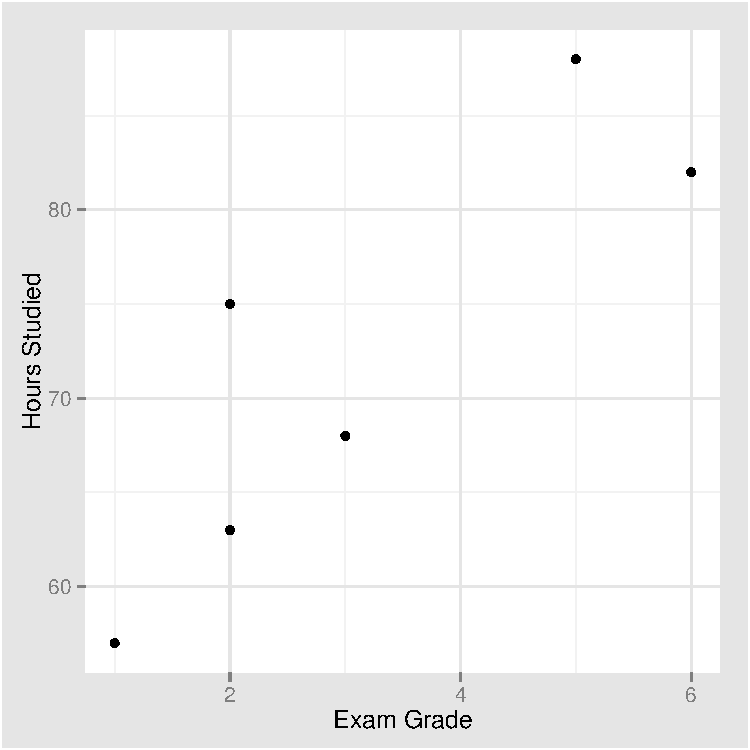
\includegraphics[width=\maxwidth]{figure/graphics-ols-1} 

}

\caption[Green regression line with prediction error, as noted in red on the chart]{Green regression line with prediction error, as noted in red on the chart}\label{fig:ols}
\end{marginfigure}


\end{knitrout}
This is very similar to the traditional algebra formula $y=mx+b$ with slope $m$ and y-intercept $b$. In this case, the slope is ${\beta}$.
\begin{equation*}
{\beta}=\frac{Cov(X,Y)}{Var(X)}=Corr(X,Y)\frac{StdDev(Y)}{StdDev(X)}
\end{equation*}

Regressing exam grade on hours studied
\begin{equation*}
{\beta}=\frac{16.3}{114.4}=0.14
\end{equation*}

The linear regression always goes through the point $(\bar{x},\bar{y})$, so returning to algebra, any point plus the slope determines the line:
\begin{equation*}
{\alpha}=\bar{y}-{\beta}\bar{x}
\end{equation*}

$\hat{\alpha}=\ensuremath{-6.91}$ for our regression.

So,
\begin{equation*}
\hat{y}=\ensuremath{-6.91} +0.14\bar{x}
\end{equation*}



The predicted value for any $y_i$ is $\hat{y_i}$, and the prediction error is $\hat{\epsilon}_i=y_i - \hat{y_i}$.

Some properties of the Simple Linear Regression:
\begin{itemize}
  \item $\Sigma_{i=1}^{N} \hat{\epsilon}_i=0 $
  \item $\Sigma_{i=1}^{N} x_i \hat{\epsilon}_i=0 $
  \item The predicted values $\hat{y_i}$ minimize the sum of the squared prediction errors, $\Sigma_{i=1}^{N} \hat{\epsilon}_i^2$, often referred to as Sum Squared Errors, or SSE.
  \item The regression equation is valid to predict $\hat{y}$ values in the range of X, that is, on the interval (min(X),max(X)), and any prediction will be in the range of (min(Y),max(Y))
\end{itemize}



\end{document}
